%%%%%%%%%%%%%%%%%%%%%%%% VRES LATEX %%%%%%%%%%%%%%%%%%%%%%%


% This sets the style of the document, you can use different built in styles, create your own .cls files or download ones from the Internet. This one is fairly standard to use
\documentclass[18pt]{article}

%%%%%%%%%%%%%%%%%%%%%%%%%%%%% Packages %%%%%%%%%%%%%%%%%%%%%%%%%%%%%%

% This package is handy for captioning figures, you can set caption style here as well
\usepackage[font={large,it}]{caption}
\usepackage[a4paper, portrait, margin=0.5in]{geometry}
% This is important for position images as latex will put your image where it best fits unless you tell it otherwise
\usepackage{float}

% If you want images this is necessary
\usepackage{graphicx}
\usepackage{subcaption}
\graphicspath{{./images}}
% You can use this to set your margin size
%\usepackage[margin=25mm]{geometry}

% Allows you to do things such as headers and footers
\usepackage{fancyhdr}

% This needs to be in here if you want to set up your document with more than one column in sections 
\usepackage{multicol}

% Here are a few packages that help with formatting equations, you may not need to use this but I find align* from amsmath particularly useful
\usepackage{amsmath,amssymb,amsthm,textcomp,amsfonts,amsthm,mathrsfs}

% Enhances Latex's cross referencing
\usepackage{cleveref}
\usepackage{hyperref}
\hypersetup{colorlinks=true}
\hypersetup{linkcolor=blue}
\usepackage{xcolor}
\usepackage{physics}
\usepackage{gensymb}
\usepackage{mathrsfs}
% Also not necessary but I find it handy when formatting arrays and matrices
\usepackage{array}
\usepackage{xfrac}

%% These packages you'll need to download a .sty file before you can use

% This allows really nice formatting for MATLAB code, it's the main plug in package that I use
\usepackage[numbered,framed]{mcode}
\usepackage{mathrsfs}
\usepackage{hyperref}
\hypersetup{colorlinks=true}
\hypersetup{linkcolor=blue}
\usepackage{xcolor}
\usepackage{physics}
\usepackage{gensymb}

%% Feel free to add any more packages you want!!!
\usepackage{indentfirst}
\usepackage{parskip} 
\setlength\parindent{0pt}
%\setlength{\parskip}{1cm plus4mm minus3mm}
\usepackage{csquotes}
\usepackage{mathtools}
\newcommand{\Lim}[1]{\raisebox{0.5ex}{\scalebox{0.8}{$\displaystyle \lim_{#1}\;$}}}

%%%%%%%%%%%%%%%%%%%%%%%%% Setup the document %%%%%%%%%%%%%%%%%%%%%%%%

\lstset{basicstyle=\scriptsize\ttfamily,breaklines=true}
\renewcommand{\thesubsection}{\thesection\alph{subsection}.}
\renewcommand{\thesubsubsection}{\indent \roman{subsubsection}}

\numberwithin{equation}{section} % Number equations within sections (i.e. 1.1, 1.2, 2.1, 2.2 instead of 1, 2, 3, 4)
\numberwithin{figure}{section} % Number figures within sections (i.e. 1.1, 1.2, 2.1, 2.2 instead of 1, 2, 3, 4)
\numberwithin{table}{section} % Number tables within sections (i.e. 1.1, 1.2, 2.1, 2.2 instead of 1, 2, 3, 4)

\newcommand{\horrule}[1]{\rule{\linewidth}{#1}} % Create horizontal rule command with 1 argument of height

\title{	
	\normalfont \normalsize 
	\textsc{Queensland University of Technology, Vacation Research Experience Scheme} \\ [25pt] 
	\horrule{0.5pt} \\[0.4cm] % Thin top horizontal rule
	\huge VI Kitchen Assistant \\ % The assignment title
	\author{Marat (Matt) Sadykov \small n9312706 \\  Customer receipt number: \small 22705821 \\ \\ Supervised by: \\ Dr. Brown Ross \\ }
	\date{\normalsize\today} % Today's date or a custom date
	\horrule{2pt} \\[0.5cm] % Thick bottom horizontal rule
}


% Headers and footers
\rhead{VRES}
\lhead{Marat (Matt) Sadykov}
\rfoot{Page \thepage}



%%%%%%%%%%%%%%%%%%%%% Begin the Actual Document %%%%%%%%%%%%%%%%%%%%%
\begin{document}
\maketitle
\renewcommand*\contentsname{Table of Contents}
\tableofcontents
\listoffigures
\newpage
\section{Executive Summary}
\section{Acknowledgements (other's assets)}	
	Virtual environment was created using several different assets form Unity Assets Store. THose are...
	
	\large kitchen Creation Kit, Kitchen Asset, MORPH3D - Evka's body and Clothes (Cyria), RTVoice\\
%===================================================%
%													%
%===============Project Overview====================%
%												    %
%===================================================%
\section{Introduction}
\subsection{Project Overview}
	This research project is focused on constructing training environment to perform some basic tasks. In particular, it establish kitchen environment, which will be supervised by Virtual Intelligent (VI)  . Using set of motion detective tools and Kinect camera tool on the top of area, VI will be able to track persons movements, provide cooking advice and follow up environment state to inform any sort of danger or thing, which may require user attention or other assistant. This tool is aimed for people with different disabilities, in order to train watch over them self, independent from other guardians. \\
		
	Virtual assistance was given a name \textit{Evka} - \textit{Enhanced Virtual Kitchen Assistant} \footnote{from a Czech language - Eva}. Her name can be translated as Eva, which will be used in majority cases. Using a hand trackers, tool markers, property or sort of thermal scanners and area content, she will be able decide the best possible to cook menu, track user activities in order not to harm anyone, track on the state of cooking process with level of heat, time and user actions. \\	
	
	At current stage Eva is able to communicate with her voice using "voice asset". Her responses are generated based on user actions. Original idea was to develop Question-Answer Virtual Intelligent environment. However, after going through limitation of the project, users ability and current level of technologies, idea was postponed to better times. \\	
	
	As a result, Eva able to use Unity Engine Kitchen environment around, which were marked with a tag depending on, which type of tool it belongs. Her dialogues stored in a tree hierarchy and changes depending on user actions. In the mean time, player has abilities to manipulate with object using controllers, represented as mouse and keyboard.
\subsection{Report Aim}
	Report is aimed to describe what limits can be overcome using game engine. It will present training idea and how easily constructed and adaptive. In the world, where Artifial Intelligence started to take place, this research may prove useful to other similar goals.\\
	
	As a result, it will contain achieved demonstration and some basic manipulation. In addition, an API document will be generated and, part which requires mentioning, applied to Methodology part.
	
\section{Background research}	
	\subsection{Problems and Solutions}
	The foundation for research was established by supervisor of the project, based on his article~\cite{quteprints100187} about Embed of VR content in life training. It highlighted several concerns, which will be difficult to overcome and suggested several solution. One which closely related to correct research are followed: \\	
	\begin{enumerate}
		\item People with intellectual disabilities finding use of keyboard and mouse harder than using joysticks. Based on P. J. Standen~\cite{control} research data, it will be logical to conclude that interaction problem must be solved within virtual world, rather than persons' abilities.
		\item Virtual training environment must be processed with guides. However according to Jen K.Y. Wu~\cite{WU20058} research data people not always react on messages or warnings around them. Use of simple Graphical User Interface (GUI) must be limited as much as possible, due to its' ineffectiveness. However, some of disabilities highlighted that person may be very precise with following instructions or commands if it's given with close person.
		\item Environment itself may cause learning challenges. Even for person without any difficulties, it is usually a bit complicated to switch between virtual world to real. Some of skills practised on simulator, not always easily achieved in practice. As an example may be given a driving test and danger, which usually comes to first time drivers. That is why driving instructors used as a guiders in both situation. With their support person may overcome fear and begging following learned skills along side with precaution instincts.
	\end{enumerate}
	Based on such limitation, solution was yet closer than anyone can think. First and the most complicated one - controllers. There are two approaches to it, first is Virtual Reality itself. Modern VR glasses requires wearing a helmet with two VR-joysticks. This way, they hands will be processed and displayed in virtual reality like their own. This way will require some training with VR, but it less limited than keyboard \& mouse and give person freedom of view and hand movements. \\
	Second approach is Augmented Reality. It will require specially established kitchen area with several sensors around and modified VR glasses. Now, person will be in the familiar area, but VI will be able to recognise objects around, draw video projection on the glasses and modify with own images, highlighting and any other information. With this approach, persons view is free from any controllers, such tools like knife, spoon, water bottle or saucepan are tracked by sensors around.\\
	Both solutions are similar to each other with own pros and cons. The goal is to develop universal solution. \\
	
	Second problem is that entire research is focused on. Except the idea of VI who watch over environment, it also must act as adviser or like people used to say a virtual friend. The whole reason for VI having a body, voice, personality is a part of training program. Person must learn to trust that men or women, so that words and tasks will make a sense for person. If people with disabilities have problems with focusing their attention on something particular, then VI person may help to overcome this dis-balance and enhance his abilities. This approach is much complicated than it sound, in order to create unpredictable behaviour will take much higher computational efforts. However, research focused on creating close demonstration.\\
	
	Third problem is something unclear from human part of view. This will be hardly hardware problem, than personal abilities. To create an environment which will suit every persons need based on his attitudes will go far ahead modern years, from physical and physiological point of view. Currently, idea was focused on some particular group of people, which were trained under certain program and may achieve same goals. \\
	
	\subsection{**Current achivements}		
	There are several companies in Australia, who already perform similar technological actions. Endeavour Fondation, doctors . Multicap. \\
	
	Experience with multicap touch that children are more attractive to robots\ldots
	Experience with multicap touch that performing basic not complicated tasks, which are easily repeatable, are easier to learn. Level of complicanse can be compared house cleaning and learning dance moves.\ldots	
	
	Endeva research results \\
	
	Use results of ~\cite{LOTAN2009229} as prove good resulting possibility. \\
	
	Those are difficulties, which current project is aimed to overcome and provide possible solution and establish ground for other modifications. \\ \\
	
	\subsection{*Development approach}
	Starting point from a designe point of view can be considered a Video Games. In the most popular gaming Library called Steam (make reference later), developers created a Job simulation, one of them is actual cooking in drawed kitchen. However, this game is focused only for (funny people), and hardly can be taking for training program. Second one is more beatufull from design point of view, but difficult for persons with intelectual disabilities. (Potion game or whatever magic thing was it). \\
	
	Game drawbacks
	\begin{enumerate}
		\item GUI environment
		\item useless assistant
		\item Unrealistic level design
		\item Envirenment does not react on player action
		\ldots
	\end{enumerate}

	This project aimed to progress this idea and bring it as close to reality as possible. \\
	
\section{Methodology}	
	\begin{enumerate}
		\item Establish Unity on Home Windows Machine. Google drive used as source control. - Unity 2017.2.0f3 - DONE
		\item Use Unity Assert Store to establish sort of kitchen environment. Kitchen asset and creation kit. MCS Female for body. RT-Voice PRO. Meximio animation.  - DONE
		\item Draw VI model and place in the kitchen.  - DONE
		\item Build one work flow hierarchy with Evka's feedback. \textbf{Camera view track}  - DONE
		\item Build an easy interactions with enum states as lift pull and collisions. - NOT an EASY
		\begin{itemize}
			\item Knife - Lift, Pull, Cut. Safe state, Danger State.  - DONE
			\item Kitchen plate - Cooled, Heating, Hot. Safe state, Danger State.  - DONE
			\item Pan/Pot - Empty, filled. Cooled, Hot.  - DONE
			\item Spoon - Cooking Tool.  - DONE
			\item Glass/Plate/Shell/Fridge - Storage.  - DONE (Partially)
		\end{itemize}
		\item Give player tho hands - keyboard/mouse. - ONE IS ENOUGH
		\item Set Cooking ingredients.  - DONE
		\begin{itemize}
			\item Vegetables - Whole, Cutted. Durty, Clean. Old, Fresh.  - DONE
			\item Meat - whole, cutted, mean. Frozen, normal.  - DEMO
			\item Rice - Dry, Cleaned. Empty/ Full. - ???
			\item Past - Empty/ Full.  - DONE
			\item Potatoes - Dry, Cleaned. Empty/ Full. - NOPE
			\item Oil - Filled, Empty.  - DONE
			\item Butter/Salt/Paper/Seasons - Yes or Null. - NOPE
		\end{itemize}
		\item SetUp Avatar restrains. I.e Do not allow take knife from working area, do not put pasta into empty Pot. \ldots  - DONE	
		
	\end{enumerate}
	
	\subsection{*Development Environment}
	GEARS***\\
	Entire designing work will be performed using Unity Game Engine. Those tools allow build realistic environment, which in future may be transformed to any supported hardware, including VR. Work will be performed on Object-Oriented C# language. Unity has own Assets Store, which contains some presets and others programmers work. In project such as this, it may become the most handy tool.
	\subsection{User Manipulators}
	Surrounding manipulation was meant to go through several different implementing processes.\\	
	At current stage, our First Person Player is supported with one hand as a mouse manipulator. They were used for testing purposes and will be reimplemented to work out with more difficult controllers. \\
	
	Next, it should have been transferred to the controllers use. Instead of having mouse or knife, person will have VR joystick, which will represent his hands. \ldots \\
	
	At final product, there will be no reasons adding controllers to persons hand, instead cameras or Kinect tool will track objects around and their movements.  Players must have augmented reality set in order to see an avatar, if necessary and all other warning, visual and audio.\\
	
	
	\subsection{Tools in the worlds}
	Using kitchen assets from the store, Figure~\ref{fig:kitchen} below represents resulted area. Avatar on the middle is an assistant, which will guide player through cooking process. 
	\begin{figure}[H]
		\centering
		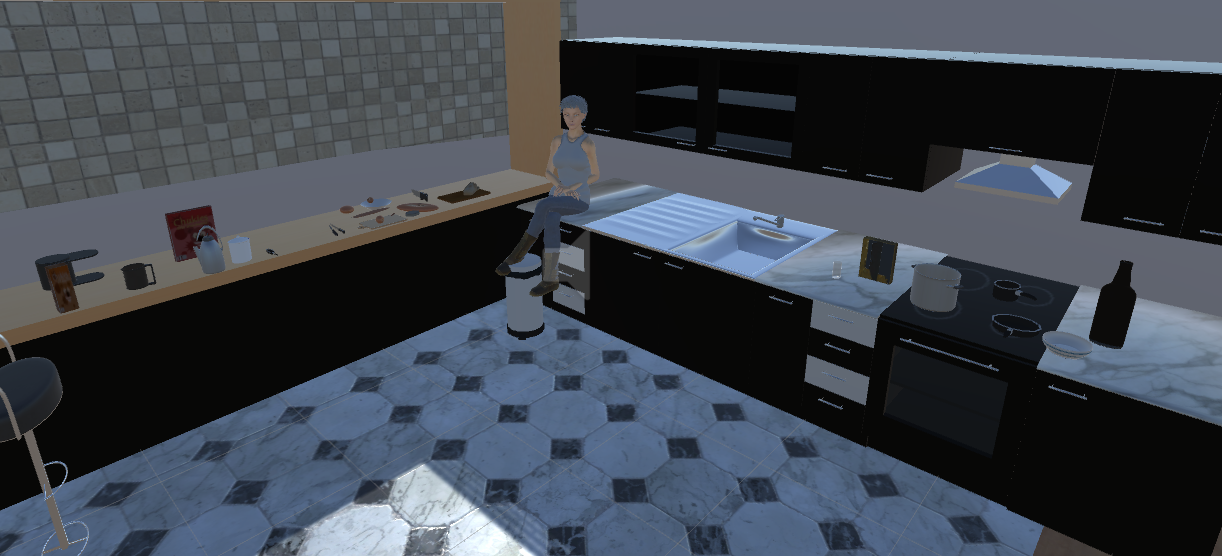
\includegraphics[width=0.7\linewidth]{images/kitchen}
		\caption{Kitchen environment}
		\label{fig:kitchen}
	\end{figure}
	
	In order to create a living representation of the world, all materials were split to different categories. Tools - knifes, spoons, and all cooking related. Ingredients - vegetables, meals, coffee, sugar, salt. Sources - Cups, Saucepans, Plates, Stoves. Their functionality follows same as in real world. \\
	This approach was chosen not only for simple process logic. It can be used for a teaching purposes, to show patients how to act with different kinds of objects. \\
	
	$ Seazing\ all\ activiries\ were\ removed.\ They require\ carefull\ logic\ approach. $
	
	In terms of the tools, they exist independently and EvKa watches over they state during entire process. They have to be always at particular area, can not be dropped and never must face to a person direction. Using a motion tracker those warning can be re-enabled. Currently, she just watch if it was dropped or not, and returns to origin location. \\
	
	Ingredients are the same as a tools, excepted that they can change their state during cooking process. They can be washed, cut, fried, frozen. Currently only few of those straits implemented. Depending on complexity of the tasks, these may be enabled. To unfroze meat, time calculates based on conditions around, vegetable can be washed after collision with water source. \\
	
	Sources are content for ingredients. Those are final stages for making food. After combining all ingredients, it calculates or sets time for cooking. After, Evka just monitors conditions and provides reminder in the cooking process. \\
	
	Those are basic tasks which person expect to do around kitchen. \\
	
	\ldots \\
	
	RTVoive capable of using Windows Mac voice and MarryTTS - adaptive served voice. Allows change sharpens, type and speed of voice acting, if necessary
	
	\subsection{Evka}
	In order to attract person attention and keep his mind occupied, Evka received a human body, which acts as a support\\adviser around kitchen. Here abilities extend at entire area, however as a person she located at place, which is on the view, but does not affects process around. She also acts as Audio Source, as basic interaction abilities like talking, greeting and idle sitting. Her skills as a person can be extended, depending how living she must be, right now she capable only to track persons view and call for his attention, then he gets distracted. \\
	\begin{figure}[H]
		\centering
		\begin{subfigure}{0.4\textwidth}
			\centering
			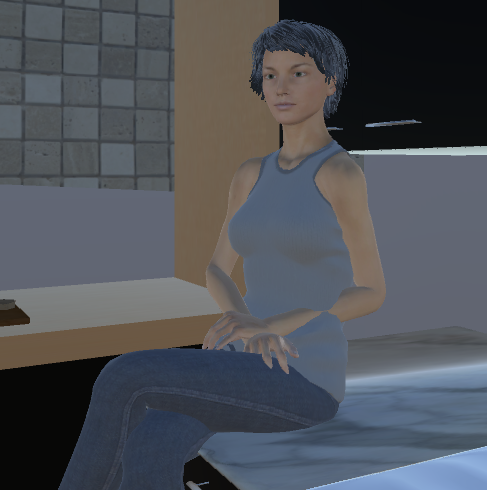
\includegraphics[width=1\linewidth]{images/Evka_sit_1}
			\caption{Evka's idle sitting}
		\end{subfigure}
		\begin{subfigure}{0.4\textwidth}
			\centering
			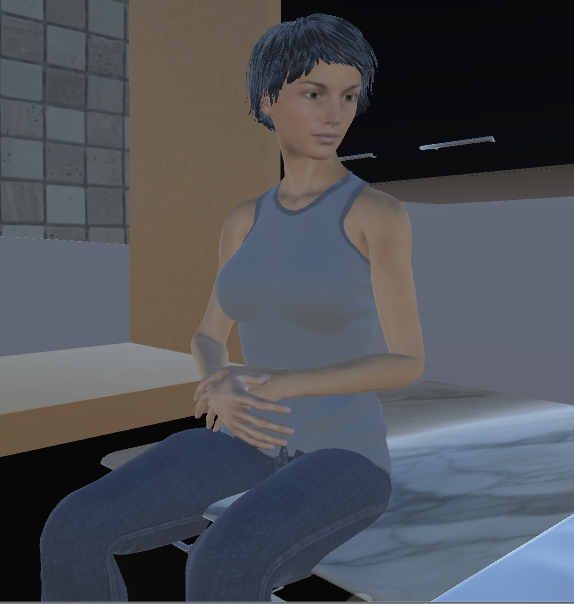
\includegraphics[width=0.96\linewidth]{images/Evka_sit_2}
			\caption{Evka's idle talking}
		\end{subfigure}		
		\caption{Evka}
		\label{fig:evkasit1}
	\end{figure}
	
	
	Currently, her voice is product of inbuilt Windows or Mac Voice, it maybe not emotional, but contains general understanding of the tasks. This approach will make sure, that patients still exist around area and occupied with cooking process. If not - she will remind him or her.
	
	
	One of the Evka's abilities is to point to the objects around. This function is used in case if person gets lost around. it can be used by simple call. \ldots
	\subsection{*Instruction}
	
	In order to demonstrate the process of easy creation of the new item in the kitchen, following instruction will be provided.\\
	
	First you have an area. Drop any item which you want to add to surrounding. Manipulate with sizes and add one of pre existed tags, $\left(\ or\ create\ a\ new\ one\ if\ necessary,\ it\ may\ require\ longer\ process\  \right) . $ \\
	
	Program will automatically apply collidors, rigidbody and transform scripts. Take for example we want to add franpan an extra tool. After adding it to a world, it will be able to store content, which called ingredients for cooking. \\
	
	Second, create a receipt. Better if it will be stored somewhere accessible. Script named $receipts$ contains all current staff possible to cook. As an example, lets create a receipt for stir-fry mince with onion cooked on the olive oil. We assume that pasta already ready and it's not part of receipt. $ \left(such\ complex\ receipts\ will\ require\ more manipulation.  \right) $ Create and Array List with strings, which contains \{"oil", "cut onion", "mince", "mixed" \}. Last word will mean that content must be stirring with any object which can do it, like spoon. Time for cooking may be calculated automatically with formulas and room conditions, or can be parsed and presented. \\
	
	Sooner or later it will be noticed that mince does not actually exist in the world. However, this is not a difficult process to perform. Drop any item which you want and add tag mince, same one you used in receipt. \\ \ldots \ldots TO BE ADDED LATER. Currently it is a buggy approach. \ldots \ldots Program will go through all kind of tag and apply general manipulations scripts. As soon as collision will be performed, object will be considered to be added to container. If cooking process requires other manipulation with object like changing a state from solid to messed, it can be performed through modefying a loop with paricular code \ldots \ldots If process requires harder manipulation, then appropriate scripts must be created and added in the same loop as Game Component. 
	
	Add all this information to following structure and pass to the methods. By default EvKa's dialogues will be set as a simple remainders, they also can be modified from this call. Basically this is a process of basic cooking. All other processes followed with other instructions. \ldots
	
	\subsection{?Logic of the world. *Strips algorithm}
	In order to understand processes which occurs around, it is better to view them separately. As it's been already discussed, it consist of 3 types of tool. Every tool type monitored by their own independent rules, which can not be broken. This designed to keep user in certain boundaries then he is not in the process of cooking something particular. This approach also allow perform some multitasking operations. All of them are united by one unique cooking process. The example approach, which was mentioned above, showed how logic is united to perform one particular task. However, EvKa can leave focus on user reaction, and focus on the states of objects around. If their condition may cause any danger - certain response will be called.
	
	Response of EvKa's reaction depends on her level of the mood. This approach makes her feel a bit as living bean, and as soon as her patience runs out, she will call for assistance from supervisor.
	
	
\section{Conclusion}
\begin{enumerate}
	\item What was achieved? - Environment designed, algorithm adaptive, dialogues created.
	\item Portability. - Extract pachage, prefab..
	\item Augemented reality research
	\item What has become with Evka
\end{enumerate}
	As a result of two months research and development, design wend through several modifications. At the end, resulting product came to VI, which able track state of the objects around, give certain feedback and serve as virtual assistant. Logic behind is easily adaptable and can be reused for other tasks around kitchen. This will totally depend on clients desire and persons abilities. \\
	
	However, this is not  guaranty total independence, but it will a first step to something greater in the future. \\
	

\section{?Proposal. Do I even need to copy it here?}	
	
	
%===================================================%
%													%
%============Bibliography and refferencing==========%
%												    %
%===================================================%

\newpage
\begin{flushleft}
\bibliographystyle{referencing/IEEEtran}
\bibliography{referencing/referenceList}

\end{flushleft}

\end{document}
